\section{Schaltregler}
\subsection{Boost-Converter}
Macht aus einer kleinen Eingangspannung eine Grosse Ausgangspannung. Grundprinzip: Spule wird mit Zeit $t_{on}$ geladen, da Spannung in Spule nicht springen kann, muss diese beim entladen ($V_L < 0$, d.h. $V_{out} > V_{in}$) durch die Diode in den Kondensator (Linearer Verlauf).
\begin{center}
	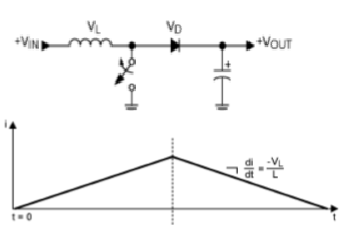
\includegraphics[width=0.6\linewidth]{Images/boost}
\end{center}
\begin{align*}
	\Delta I_{L_{on}} &= \frac{V_{in}}{L}\cdot t_{on} \\
	\Delta I_{L_{off}} &= \frac{V_{in} - V_{out}}{L}\cdot t_{off} \\
	\Delta I_{L_{on}} &\eqi - \Delta I_{L_{off}} \qquad \text{(Gleichgewicht, wenn eingeschwungen)} \\
	V_{out} &= V_{in} \cdot \underbrace{\left(1 + \frac{t_{on}}{t_{off}}\right)}_{=\frac{1}{\text{Duty Cylce}}}
\end{align*}
\textbf{Achtung:} DutyCycle $d = \frac{t_{on}}{t{on} + t{off}}$ immer überprüfen, um korrekten Faktor zu erhalten.\\
Die Energie des Lastwiderstandes $E_{Load} = \frac{V_{out}^2}{R_{Load}}T_{clk}$, wobei $T_{clk}$ der komplette Taktzyklus ist, muss mindestens von der Spule geliefert werden. Die Energie der Spule lässt sich durch $E_L = \frac{L}{2} {i_L}^2$ und des Kondensators $E_c = \frac{C}{2}{V_c}^2$ berechnen.

\subsection{Buck-Converter}
Macht aus grossen Eingangspannungen kleine Ausgangsspannungen. Grundprinzip: Schalter geschlossen, Strom steig über Spule, sobald wieder offen, Strom sinkt. LC macht einen Tiefpass-Filter und glättet DC Ausgang.
\begin{center}
	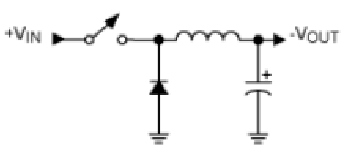
\includegraphics[width=0.4\columnwidth]{Images/buck}
\end{center}
\begin{align*}
	\Delta I_{L_{on}} &= \frac{V_{in} - V_{out}}{L}\cdot t_{on} \\
	\Delta I_{L_{off}} &= -\frac{V_{out}}{L}\cdot t_{off} \\
	\Delta I_{L_{on}} &\eqi - \Delta I_{L_{off}} \qquad \text{(Gleichgewicht, nach einschingung)} \\
	V_{out} &= V_{in} \cdot \underbrace{\left(\frac{t_{on}}{t_{on} + t_{off}}\right)}_{=\text{Duty Cylce}}
\end{align*}

\subsection{Invertierender Converter}
Kombination aus Buck und Boost Converter
\begin{center}
	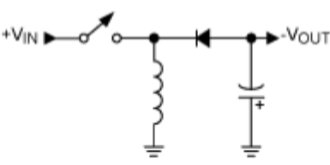
\includegraphics[width=0.4\columnwidth]{Images/inverter}
\end{center}
\begin{align*}
	\Delta I_{L_{on}} &= \frac{V_{in}}{L}\cdot t_{on} \\
	\Delta I_{L_{off}} &= -\frac{V_{out}}{L}\cdot t_{off} \\
	\Delta I_{L_{on}} &\eqi - \Delta I_{L_{off}} \qquad \text{(Gleichgewicht, wenn eingeschwungen)} \\
	V_{out} &= -V_{in} \cdot \underbrace{\frac{t_{on}}{t_{off}}}_{=\text{Duty Cylce}}
\end{align*}

\subsection{Flyback}
Auch SEPIC-Wandler können Step-up und Step-Down sein.
\begin{center}
	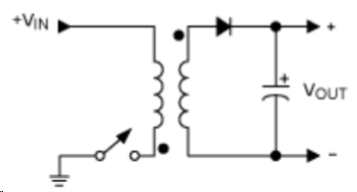
\includegraphics[width=0.4\columnwidth]{Images/flyback}
\end{center}

Beispiel für SEPIC-Wandler:
\begin{center}
	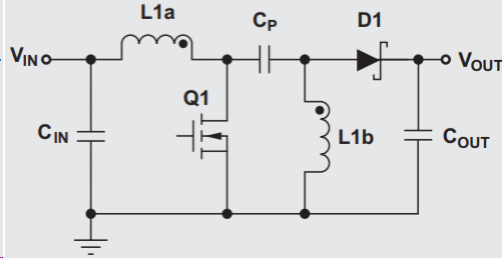
\includegraphics[width=0.6\columnwidth]{Images/sepic}
\end{center}
\begin{enumerate}[nosep]
	\item Phase Q1 geschlossen, D inaktiv
	\item Phase Q1 offen, D1 leitet
	\item Phase Schwingung
\end{enumerate}
\begin{align*}
	\text{(1)  } & \Delta I_{L1a_{on}} = \frac{V_{in}}{L1a}\cdot t_{on}\\
	\text{(2)  } & \Delta I_{L1a_{off}} = -\frac{V_{out}}{L1a}\cdot t_{off}\\
	\text{(3)  } & \Delta I_{L1a_{on}} \eqi  \Delta I_{L1a_{off}}\\
	& V_{out} = V_{in} \cdot \frac{t_{on}}{t_{off}}
\end{align*}
